\documentclass{beamer}

\usepackage{beamerthemesplit}
\usepackage{wrapfig}
\usetheme{SPbGU}
\usepackage{pdfpages}
\usepackage{amsmath}
\usepackage{cmap} 
\usepackage[T2A]{fontenc} 
\usepackage[utf8]{inputenc}
\usepackage[english,russian]{babel}
\usepackage{indentfirst}
\usepackage{amsmath}
\usepackage{tikz}
\usepackage{multirow}
\usepackage[noend]{algpseudocode}
\usepackage{algorithm}
\usepackage{algorithmicx}
\usetikzlibrary{shapes,arrows}
\usepackage{fancyvrb}
\newtheorem{rutheorem}{Теорема}
\newtheorem{ruproof}{Доказательство}
\newtheorem{rudefinition}{Определение}
\newtheorem{rulemma}{Лемма}
\beamertemplatenavigationsymbolsempty
\usepackage{textcomp}
\usepackage{graphicx}

\def \fstar {F$\ast$}
\def \fsharp {F$\#$}

\title[Верификация в коде]{Разработка инструмента\\
        для добавления статической верификации в код}
% То, что в квадратных скобках, отображается в левом нижнем углу. 
\institute[СПбГУ]{
Санкт-Петербургский государственный университет } % \\
% Кафедра системного программирования }

% То, что в квадратных скобках, отображается в левом нижнем углу.
\author[Маллабаев Азамат]{Маллабаев Азамат Нурмухамадович, 143 группа \\
  % У научного руководителя должна быть указана научная степень
  \and
    {\bfseries Научный руководитель:} ст.пр. Григорьев Семён Вячеславович}
  % Для курсовой не обязателен. Должна быть указана должность или ученая степень
  % \and
  %    {\bfseries Рецензент:} программист ООО ``Рога и копыта'' И.И. Иванов}

\date{19 мая 2016г.}

\definecolor{orange}{RGB}{179,36,31}

\begin{document}
{
% Лого университета или организации, отображается в шапке титульного листа
\begin{frame}
  \begin{center}
  {
\includegraphics[width=1cm]{pictures/SPbGU_Logo.png}}
  \end{center}
  \titlepage
\end{frame}
}
            
\begin{frame}
  \transwipe[direction=90]
  \frametitle{Введение}
  \begin{itemize}
    \item Тестирование --- доказательство некорректности программы
    \item Верификация --- доказательство корректности программы
    \begin{itemize}
       \item Статическая --- во время компиляции
       \item Динамическая --- во время выполнения
    \end{itemize}
  \end{itemize}
\end{frame}

\begin{frame}
  \transwipe[direction=90]
  \frametitle{Инструменты верификации}
  \begin{itemize}
    \item AutoProof --- верификатор языка Effel
    \item Coq --- интерактивное средство для доказательства теорем
    \item \fstar~--- язык с поддержкой верификации
    \begin{itemize}
      \item ML-подобный, каким также является \fsharp
      \item Работает в DotNet
      \item Транслируется в \fsharp~без учета ограничений
    \end{itemize}
    \item Z3 --- низкоуровневый инструмент верификации
  \end{itemize}
\end{frame}

\begin{frame}[fragile]
  \transwipe[direction=90]
  \frametitle{Атрибуты}
  \textbf {Атрибуты} --- поля, применимые к элементам программы
  
  \textbf {}
  
  \textbf{Атрибуты в \fsharp}
  \begin{verbatim}
 1 [<Obsolete("Код -- баян")>] //устаревший метод
 2 [<EntryPoint>] //атрибут начала программы
 3 let helloSayer () = //метод, к которому применены атрибуты
 4    printfn "Hello, world!!!"
  \end{verbatim}
\end{frame}

% Обязательный слайд: четкая формулировка цели данной работы и постановка задачи
% Описание выносимых на защиту результатов, процесса или особенностей их достижения и т.д.
\begin{frame}
  \transwipe[direction=90]
  \frametitle{Постановка задачи}
  \textbf{Цель:} разработка инструмента для добавления статическиой верификации в код на \fsharp~с использованием верификатора \fstar
  
  \textbf{Задачи}
  \begin{itemize}
    \item Изучить компилятор \fsharp~и верификатор \fstar
    \item Разработана архитектура системы
    \item Разработать транслятор подмножества \fsharp~в \fstar
  \end{itemize}
  
\end{frame}

\begin{frame}
  \transwipe[direction=90]
  \frametitle{Аритектура инструмента}
  \center
  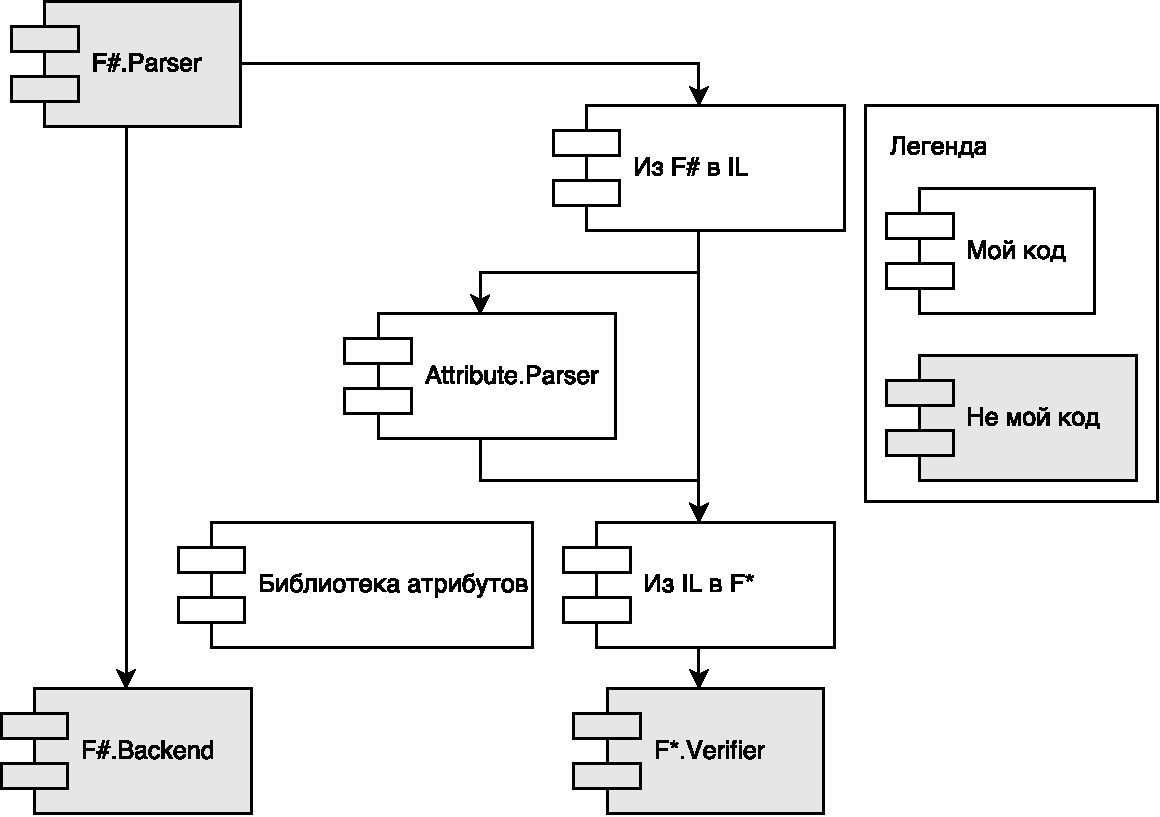
\includegraphics[width=0.9\linewidth]{Teh}
\end{frame}

%\begin{frame}
%  \transwipe[direction=90]
%  \frametitle{Сценарий использования и работы транслятора}
%  \center
%  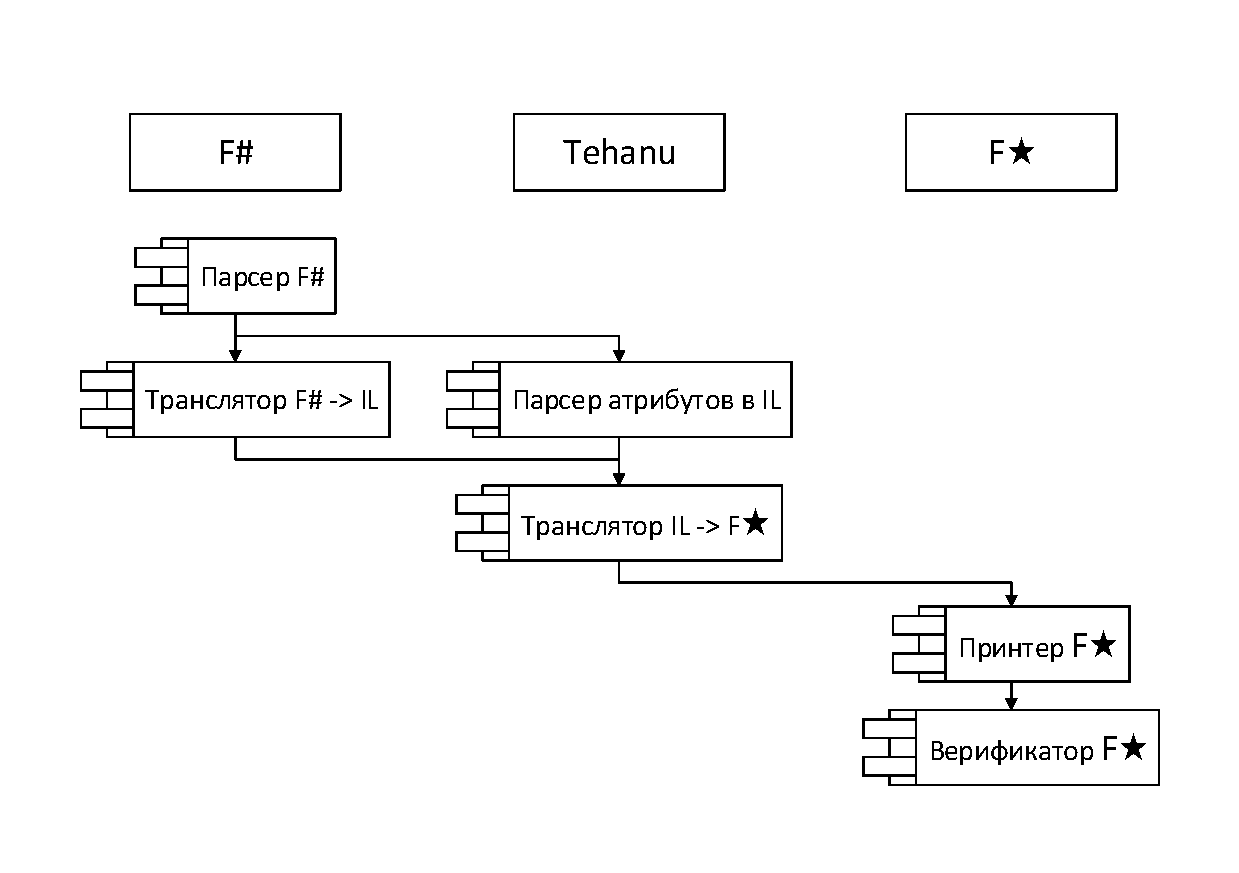
\includegraphics[width=0.9\linewidth]{TehanuStruct}
%\end{frame}

\begin{frame}[fragile]
  \transwipe[direction=90]
  \frametitle{Поддерживаемые выражения}
  \begin{itemize}
    \item Модули
    \item Типизированное опрделение функции
    \item Условный оператор if-then-else
    \item Применение функции
    \item Бинарные операции
    \item Целые числа
    \item Выражения верификации forall и exist
  \end{itemize}
\end{frame}

\begin{frame}[fragile]
  \transwipe[direction=90]
  \frametitle{Пример использования атрибута верификации}
  \begin{verbatim}
 ///Верифицируемая функция
 1 [<Total("forall x y . x < y ==> i x + 2 <= i y")>]
 2 let f (x: int): int =
     if x > 1
     then x * x * x
     else x - 2 
 
 
 //Неверифицируемая функция
 1 [<Total("forall x y . x < y ==> i x < i y")>]
 2 let g (x: int): int = x * x
  \end{verbatim}
\end{frame}

\begin{frame}
  \transwipe[direction=90]
  \frametitle{Результаты}
  \begin{itemize}
    \item Изучены компилятор \fsharp~и верификатор \fstar
    \item Разработана архитектура системы
    \item Разработан транслятор из подмножества \fsharp~в \fstar
  \end{itemize}
\end{frame}

\end{document}
